%======== BEGIN inserted by add_gemeinsam.rb ======================
\documentclass{beamer}
\usepackage[german]{babel}
\usepackage[T1]{fontenc}
%\usepackage[latin1]{inputenc} 
\usepackage[utf8x]{inputenc}

\usepackage{verbatim} 
\usepackage{listings} 

% \lstset{numbers=left, numberstyle=\tiny, numbersep=5pt} 
\logo{
\includegraphics[width=0.7cm]{../images/ruby.png}}

%\usetheme{Warsaw}
%\usetheme{Hannover}
%\usetheme{PaloAlto}
%\usetheme{JuanLesPins}
%\usetheme{Antibes}
%\usetheme{Shingara}
%\usetheme{Berlin}
%\usetheme{Oxygen}
\usetheme{Singapore}

\usecolortheme{beaver}
% albatross | beaver | beetle |
% crane | default | dolphin |
% dove | fly | lily | orchid |
% rose |seagull | seahorse |
% sidebartab | structure |
% whale | wolverine


\title[Ruby]{Programmiersprache Ruby}
\author{Sven Suska, Thomas Preymesser}
%\institute{}
\date{2009-Juli-2}


\usepackage{tikz}
\usetikzlibrary{arrows,shapes,decorations}


\tikzstyle{klasse} = [rectangle, draw, thin, fill=blue!20 ]
\tikzstyle{objekt} = [ellipse, draw, thin, fill=green!20, minimum height=2.5em]

\tikzset{%
    class/.style={green,>=triangle 45}
    }
\tikzset{%
    eigenc/.style={very thin,green,>=triangle 45}
    }
\tikzset{%
    superc/.style={thick,red,>=open triangle 45}
    }
\tikzset{%
    method1/.style={thin,blue,bend left=45,to reversed->}
    }
\tikzset{%
    method1r/.style={thin,blue,bend right=45,to reversed->}
    }
\tikzset{%
    methods/.style={thin,blue,bend left=45}
    }

\newcommand{\klassebox}[2]{\begin{tabular}{l}{\it #1} \\ \hline \tt{#2}\end{tabular}}

\newcommand{\bls}[1]{{\bf\lstinline{#1}}}

\begin{document}
\lstset{language=Ruby}
\lstset{basicstyle=\small,numbers=none, numberstyle=\tiny, numbersep=5pt}
%======== END inserted by add_gemeinsam.rb ======================
\begin{frame}
  \frametitle{FXRuby}
  \begin{itemize}
    \item Cross Platform GUI Library
    \item Basierend auf FOX Toolkit, geschrieben in C++
    \item http://www.fxruby.org/ (Buch f"ur FXRuby erh"altlich)
  \end{itemize}
\end{frame}

\begin{frame}
  \frametitle{FXRuby / Skelett einer Anwendung}
  \lstinputlisting[frame=single,caption={beispiel1.rb}]{code/beispiel1.rb}
\end{frame}

\begin{frame}
  \frametitle{FXRuby / Skelett einer Anwendung}
  \begin{figure}
    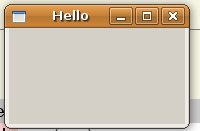
\includegraphics[scale=1.0]{code/beispiel1.jpg} 
    \caption{Einfachste Anwendung}
  \end{figure}
\end{frame}

\begin{frame}
  \frametitle{FXRuby / Buttons}
  \lstinputlisting[frame=single,caption={beispiel2.rb}]{code/beispiel2.rb}
\end{frame}

\begin{frame}
  \frametitle{FXRuby / Buttons}
  \begin{figure}
    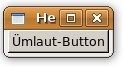
\includegraphics[scale=1.0]{code/beispiel2.jpg} 
    \caption{Buttons}
  \end{figure}
\end{frame}

\begin{frame}
  \frametitle{FXRuby / Buttons + Messages}
  \lstinputlisting[frame=single,caption={messages.rb}]{code/messages.rb}
\end{frame}

\begin{frame}
  \frametitle{FXRuby / Tooltips}
  \lstinputlisting[frame=single,caption={tooltip.rb}]{code/tooltip.rb}
\end{frame}

\begin{frame}
  \frametitle{FXRuby / Tooltips}
  \begin{figure}
    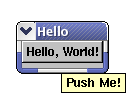
\includegraphics[scale=1.0]{code/hello-with-tooltip.png} 
    \caption{Tooltips}
  \end{figure}
\end{frame}

\begin{frame}
  \frametitle{FXRuby / M"oglichkeiten}
  \begin{itemize}
    \item Icons/Bilder auf Buttons
    \item Men"us
    \item Daten in Clipboard schreiben / lesen
    \item Drag and Drop
    \item Dialogboxes (modal und non-modal)
    \item Directory-Trees
    \item Muliple-Document-Interface (MDI)
    \item Group-Boxes
    \item Shutter
  \end{itemize}
  ... und zahllose andere Features. Weitere Beispiele unter \href{http://www.fxruby.org/doc/examples.html}{http://www.fxruby.org/doc/examples.html}.

\end{frame}

%======== BEGIN inserted by add_gemeinsam.rb ======================
\end{document}
%======== END inserted by add_gemeinsam.rb ======================
